\documentclass[11pt]{article}
\usepackage[a4paper,margin=2.5cm]{geometry}
\usepackage[T1]{fontenc}
\usepackage[utf8]{inputenc}
\usepackage{amsmath,amssymb}
\usepackage{booktabs,array}
\usepackage{graphicx}
\usepackage{xcolor}
\usepackage[numbers,sort&compress]{natbib}
\usepackage[colorlinks=true,linkcolor=blue!50!black,citecolor=blue!50!black,urlcolor=blue!50!black]{hyperref}
\graphicspath{{./}}

\newcommand{\qgZ}{qg_Z}

\title{When does a three-level readout help?\\
Leakage flags, erasure qubits and the qg T1-aware decoder}
\author{Vicente Humberto Monteverde\\
\small Universidad del Museo Social Argentino (UMSA), Argentina\\
\small ORCID 0000-0001-8884-4811}
\date{\small Draft of 29 September 2026; revised 30 September 2026}

\begin{document}
\maketitle

\begin{abstract}
Transmon qubits leak to their second excited state, and a three-level readout can flag it. We ask
whether this helps the qg T1-aware decoder, a minimum-weight matching decoder whose weights follow the
final data readout and which a register-mean polar-bias witness switches on only when relaxation
dominates~\cite{monteverde2026qang,monteverde2026witness}. Six simulated tests on a circuit-level
surface-code memory, each with its criterion fixed before the reported run, give a consistent answer.
(i) When a leaked qubit keeps its value, erasing flagged qubits makes every decoder worse, and the
whole qg gain (1.68$\times$) comes from the qubit-level reweighting. (ii) When leakage scrambles the
value, the flag and the reweighting combine better than either alone: 1.68$\times$ over the best
leakage-aware decoder at distance 3. (iii) A Bayesian weight for the flag, a flip probability
$a/(1+a)$ with $a$ the leak asymmetry between $|0\rangle$ and $|1\rangle$, contains both cases, is
never worse than ignoring leakage, and is not uniformly better than erasure (one of four predictions
fails). The combined gain grows with distance, from 1.48$\times$ to 1.77$\times$. (iv) A coherent
three-level simulation of a diabatic CZ gives $a=0$ and a leaked qubit that keeps its value and still
flips its ancilla with probability 0.97. For such transmons the flag is useless, erasure hurts, and the
qg gain (1.81$\times$ at $d=3$, 2.02$\times$ at $d=5$) needs no qutrit readout. (v) On erasure qubits, which herald T1 decays as they happen, a naive
combination with qg is harmful when heralding is good (0.46$\times$ at heralding efficiency
$h=0.99$); scaling the prior of unheralded decays by $1-h$, a rule then tested with its own
pre-registration, removes the loss and keeps a gain of 1.41--1.68$\times$ at $h=0.5$. All results are
simulations, reproduced by scripts and pinned by regression tests.
\end{abstract}

\section{The question}

The qg unit describes a qubit by its polar bias $\qgZ=\langle\sigma_z\rangle$ and related
quantities~\cite{monteverde2026qang}. In a surface-code memory, relaxation (T1) biases the final data
readout towards $0$; a companion preprint~\cite{monteverde2026witness} uses this to reweight the
matching graph shot by shot (a data qubit read as 1 has not decayed, so its decay faults are
discounted), and switches the reweighting on only when the register-mean $\qgZ$ of a calibration batch,
divided by the detector rate, exceeds 1. We call this the qg decoder.

Superconducting qubits also leak out of the computational space, mainly to $|2\rangle$, and leakage is
a known threat to error correction~\cite{aliferis2007leakage,suchara2015leakage,mcewen2021leakage}. A
three-level readout can see it, and leakage-aware decoders treat flagged qubits as
erasures~\cite{suchara2015leakage,wu2022erasure,varbanov2020leakage}. Before extending qang beyond
qubits we asked a narrow question: does the qg decoder gain anything from a three-level readout,
beyond what standard leakage handling already gives? The rule agreed in advance was to extend qang
only if it does.

\section{Setup}

\paragraph{Memory and noise.} A rotated surface code in a Z-memory experiment, distance $d=3$ with 3
rounds or $d=5$ with 5 rounds, simulated shot by shot at circuit level. Noise: two-qubit depolarizing
$p_2$ after each CNOT, amplitude damping $\gamma$ per layer (twice during measurement), readout flips
$q$. Two regimes: T1-dominated ($p_2=0.0005$, $\gamma=0.003$, $q=0.002$) and depolarizing
($p_2=0.004$, $\gamma=0.0005$, $q=0.002$).

\paragraph{Leakage.} After a CNOT a data qubit leaks with probability $\ell=0.002$ if it is in
$|1\rangle$ and $a\ell$ if it is in $|0\rangle$. A leaked control kicks its ancilla with probability
$\kappa$ (1/2 unless stated), does not decay, and returns with probability $r$ per layer. Three
choices define a model: the asymmetry $a$, the value it returns to (always $1$, or random), and how a
two-level readout assigns $|2\rangle$ (as $1$, or at random). The final three-level readout flags every
qubit still leaked.

\paragraph{Decoders.} All use minimum-weight perfect matching (PyMatching~\cite{higgott2022pymatching})
on the same detector graph: \emph{standard} (leakage ignored); \emph{erasure} (the final-readout edges
of a flagged qubit get probability $1/2$, or, where stated, all its edges); \emph{Bayesian weight}
(Section~\ref{sec:bayes}); \emph{qg} (the T1 reweighting); and the combinations qg + erasure and
qg + Bayesian weight. Decoders are compared on the same shots with a paired (McNemar) $z$.

\paragraph{Protocol.} Each test states its criterion in the script before the run. For the last five,
script and criterion were committed to the public repository before the reported run
(commits \texttt{3fa4d63}, \texttt{daf0b6f}, \texttt{092580f}, \texttt{e877a72}, \texttt{68d8d00}),
and the code was debugged on a different seed.

\section{Results}

\subsection{A leaked qubit that keeps its value: a negative result}

In the first model ($a=0$, return to $1$, $|2\rangle$ read as 1, $r=0.05$) we compared qg + erasure with
erasure. The criterion (1.3$\times$, $z\ge3$, never worse) formally passed with 1.65$\times$
($z=+14.8$), but the pass was an artefact (Table~\ref{tab:neg}). The erasure baseline, which erased a
flagged qubit's whole history, was worse than ignoring leakage in every regime ($z=-3.8$ to $-6.0$).
The qg decoder \emph{without} any flag beat standard by 1.68$\times$ ($z=+14.7$), and adding flags to it
made it worse ($z$ between $-2.8$ and $-4.9$). Erasing only the last layer, a variant added after the
first run, was less harmful but still worse than standard. The reason is simple: a qubit that leaks only
from $|1\rangle$ and returns to $|1\rangle$ is read correctly as 1, so declaring it erased discards a
right value. We recorded a negative result.

\begin{table}[t]
\centering\small
\caption{Logical error, first model ($a=0$, value kept), $d=3$, 60\,000 shots per regime.}
\label{tab:neg}
\begin{tabular}{lcccc}
\toprule
regime (witness) & standard & erasure & qg + erasure & qg, no flags\\
\midrule
leakage + T1-dominated (1.68) & 0.0156 & 0.0165 & 0.0100 & 0.0093\\
leakage + mixed (1.27) & 0.0099 & 0.0106 & 0.0089 & 0.0084\\
leakage + depolarizing (0.34) & 0.0032 & 0.0036 & 0.0036 & 0.0032\\
strong leakage, depolarizing (0.46) & 0.0021 & 0.0032 & 0.0032 & 0.0021\\
\bottomrule
\end{tabular}
\end{table}

\subsection{Leakage that scrambles the value}

An exploratory rerun suggested that the flag helps when the leaked qubit loses its value. We then fixed
a second model and a stricter criterion before the run: leakage from $|1\rangle$ ($\ell$) and from
$|0\rangle$ ($\ell/2$), return to a random bit, $|2\rangle$ read at random, and per-round leakage
flags with efficiency 0.8. The criterion required the qg decoder with flags to beat the \emph{better}
of two leakage-aware decoders by $\ge1.3\times$ with $z\ge3$ in some regime, never lose with
$z\le-3$, and the flags to improve qg in every regime.

Both parts passed. In the T1-dominated regime qg + flags reached 0.0106 against 0.0177 for the best
leakage-aware decoder (1.68$\times$, $z=+15.3$), and 1.28$\times$ in the mixed regime; the flags
improved qg in all four regimes ($z=+4.0$ to $+8.9$). The combination is more than the product of its
parts: flags alone gave 1.07$\times$ over standard, the reweighting alone 1.45$\times$, together
1.78$\times$. A plausible mechanism is that the reweighting trusts the final data bits, and a
leaked qubit's final bit is random, so erasing it removes a misleading input. A second seed gave
1.43$\times$ ($z=+11.3$). Per-round detection added little at $d=3$: with the final readout alone the
gain was 1.39$\times$.

\subsection{A rule for the flag}\label{sec:bayes}

The two results disagree because both erase the flag regardless of where the leak came from. If a
qubit leaks from $|1\rangle$ with probability $\ell$ and from $|0\rangle$ with $a\ell$, and is seen in
$|2\rangle$, its value before leaking was 1 with posterior $1/(1+a)$ (uniform prior). The Bayesian weight
therefore reports the flagged qubit as 1 and gives its final-readout edges the flip probability
\begin{equation}\label{eq:pflag}
p_{\rm flag}=\max\!\left(\frac{a}{1+a},\,q\right),
\end{equation}
with a neutral T1 weight, since a leaked qubit does not decay. At $a=0$ it trusts the flag's value;
at $a=1$ it is plain erasure. The first model is the case $a=0$, where the rule reduces to the
standard decoder.

We tested four predictions over five models ($M_0$, the first model; $M(a)$ with
$a=0$, $0.25$, $0.5$ or $1$, random return and random readout; $M(0.5)$ is the second model), both
regimes at $d=3$ and four models at $d=5$ (Table~\ref{tab:bayes}, Fig.~\ref{fig:leak}).
\textbf{P1} (never worse than standard) passed: $z$ from $0.0$ to $+9.0$, while erasure lost to standard
in $M_0$ ($z=-5.7$). \textbf{P2} (beats erasure for $a\le0.25$ in both regimes) failed: it held in the
T1-dominated regime ($z=+6.1$, $+7.0$, $+3.9$) but not in the depolarizing one ($+2.9$ for $M_0$,
$-0.4$ for $M(0.25)$), and at $a=0.5$ depolarizing erasure was slightly better ($z=-2.2$); the
differences are at most 5\%. A leaked qubit also scrambles its ancillas for several rounds, which the
posterior on its value ignores. \textbf{P3} (qg + Bayesian weight never worse than qg + erasure) passed.
\textbf{P4} (a qg + flag gain of $\ge1.3\times$ at both distances in $M(0.5)$) passed, and the gain
grew: 1.48$\times$ ($z=+12.5$) at $d=3$, 1.77$\times$ ($z=+13.6$) at $d=5$, and 1.55--2.11$\times$
across the four $d=5$ models. As pre-registered, with P2 failing the rule counts as partly confirmed.

\begin{table}[t]
\centering\small
\caption{Logical error in the T1-dominated regime, 60\,000 shots per point. $p_{\rm flag}$ from
Eq.~\eqref{eq:pflag}.}
\label{tab:bayes}
\setlength{\tabcolsep}{3.4pt}
\begin{tabular}{clcccccccc}
\toprule
$d$ & model & $p_{\rm flag}$ & standard & erasure & Bayesian & qg & qg + erasure & qg + Bayesian\\
\midrule
3 & $M_0$ & 0.002 & 0.0154 & 0.0163 & 0.0153 & 0.0091 & 0.0097 & 0.0093\\
3 & $M(0)$ & 0.002 & 0.0177 & 0.0171 & 0.0161 & 0.0104 & 0.0105 & 0.0099\\
3 & $M(0.25)$ & 0.200 & 0.0182 & 0.0175 & 0.0170 & 0.0119 & 0.0112 & 0.0110\\
3 & $M(0.5)$ & 0.333 & 0.0189 & 0.0181 & 0.0180 & 0.0137 & 0.0122 & 0.0121\\
3 & $M(1)$ & 0.500 & 0.0202 & 0.0192 & 0.0192 & 0.0171 & 0.0140 & 0.0140\\
5 & $M_0$ & 0.002 & 0.0100 & 0.0103 & 0.0100 & 0.0045 & 0.0049 & 0.0047\\
5 & $M(0)$ & 0.002 & 0.0118 & 0.0112 & 0.0109 & 0.0055 & 0.0053 & 0.0052\\
5 & $M(0.5)$ & 0.333 & 0.0141 & 0.0131 & 0.0131 & 0.0085 & 0.0073 & 0.0074\\
5 & $M(1)$ & 0.500 & 0.0170 & 0.0153 & 0.0153 & 0.0125 & 0.0098 & 0.0098\\
\bottomrule
\end{tabular}
\end{table}

\begin{figure}[t]
\centering
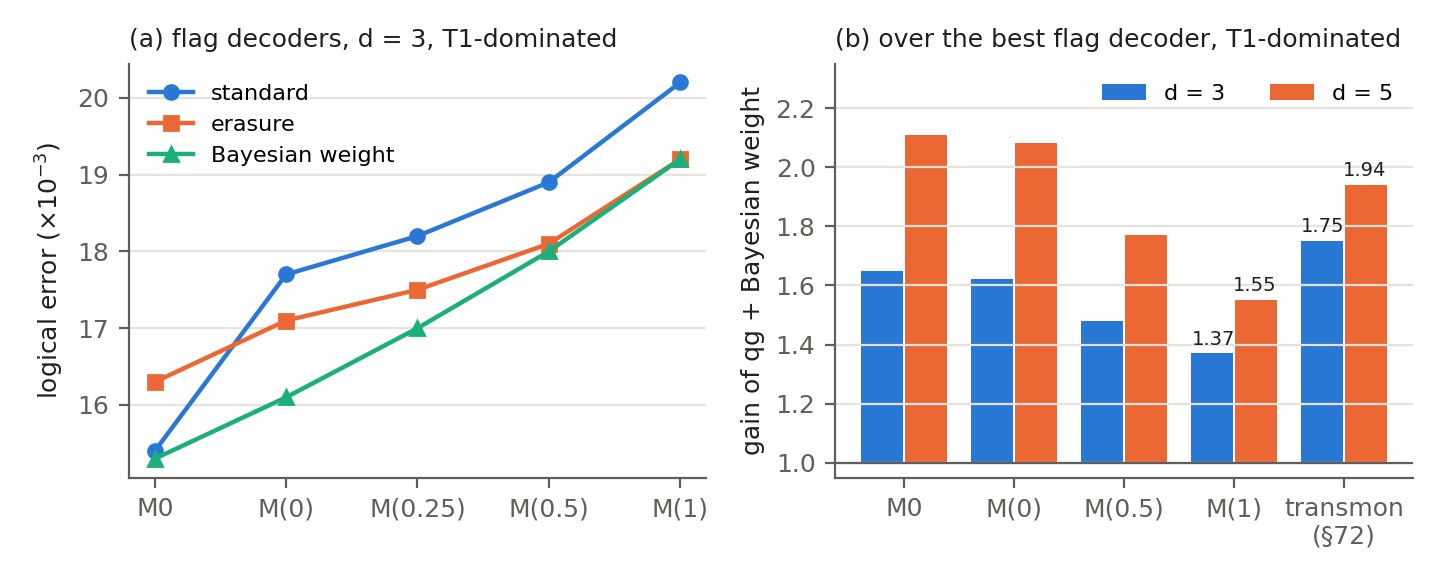
\includegraphics[width=\linewidth]{fig_leakage.png}
\caption{(a) Logical error of the three flag decoders across the leakage models, $d=3$, T1-dominated
regime. (b) Gain of qg + Bayesian weight over the better of erasure and Bayesian weight, at $d=3$ and
$d=5$, including the transmon channel of Section~\ref{sec:transmon}.}
\label{fig:leak}
\end{figure}

\subsection{Where a transmon sits}\label{sec:transmon}

The parameters of the models above were chosen, not derived. We derived them for a transmon from a
coherent simulation: two transmons truncated at three levels (anharmonicity $-2\pi\cdot0.3$\,GHz,
coupling $2\pi\cdot10$\,MHz) and a diabatic flux-pulse CZ through the $|11\rangle\leftrightarrow|20\rangle$
resonance~\cite{dicarlo2009}, with the hold time optimised for gate fidelity after virtual-Z
corrections. The gate reached an average fidelity of 0.99967 with leakage $5.4\times10^{-4}$ from
$|11\rangle$ and exactly zero from the other inputs, so $a=0$. This is structural: the exchange
coupling conserves the number of excitations, and only $|11\rangle$ can reach $|20\rangle$. A leaked data
qubit gives its ancilla a conditional phase of $0.89\pi$, so in a CNOT it still flips the ancilla with
probability $\kappa=0.97$, almost as if it were in $|1\rangle$; and it decays back to $|1\rangle$ at twice
the T1 rate. The leaked transmon is nearly invisible to its stabilizers and keeps its value: the $M_0$
corner of the map.

With this channel in the memory (and $|2\rangle$ read as 1), all four predictions made before the run
passed (Table~\ref{tab:transmon}). The Bayesian weight tied with standard (1.001$\times$, 1.011$\times$,
0.998$\times$; $|z|\le1.4$), erasure hurt ($z=-7.2$, $-4.9$, $-5.7$), and the qg decoder without flags
gained 1.81$\times$ ($z=+15.3$) at $d=3$ and 2.02$\times$ ($z=+12.4$) at $d=5$. Adding the flag to qg
cost a little, because the flagged qubit's T1 weight is set to neutral although its bit is right.

\begin{table}[t]
\centering\small
\caption{Logical error with the leakage channel derived for a transmon CZ, 60\,000 shots per point.}
\label{tab:transmon}
\begin{tabular}{clcccc}
\toprule
$d$ & regime (witness) & standard & erasure & Bayesian & qg\\
\midrule
3 & T1-dominated (1.68) & 0.0153 & 0.0163 & 0.0153 & 0.0084\\
3 & depolarizing (0.34) & 0.0031 & 0.0035 & 0.0030 & 0.0031\\
5 & T1-dominated (2.30) & 0.0079 & 0.0084 & 0.0079 & 0.0039\\
\bottomrule
\end{tabular}
\end{table}

\subsection{Erasure qubits}\label{sec:erasure}

Erasure qubits, such as dual-rail transmons~\cite{kubica2023erasure} and atoms with erasure
conversion~\cite{wu2022erasure}, herald decay events as they happen. If heralding were perfect, the
final-readout bias that the qg decoder uses would carry nothing extra. We modelled this on the same
memory without leakage: every data-qubit decay $1\to0$ is heralded with probability $h$ at its exact
location, and the erasure decoder sets that edge to probability $1/2$.

The first test predicted that the gain of qg + erasure over erasure would fall with $h$ (it did: from
1.59$\times$ and 2.04$\times$ at $h=0$ to below 1.1$\times$ at $h=0.99$) and that the combination would
never be worse than erasure alone. The last prediction failed, and the failure is the finding: at
$h=0.99$ qg + erasure reached only 0.46$\times$ ($z=-6.7$) at $d=3$ and 0.22$\times$ at $d=5$. The
T1 reweighting assumes every decay is unheralded; with heralds, a 0 at the final readout is mostly
explained already, and the reweighting counts it twice. The witness does not catch this, because the
readout bias is still there at every $h$.

An exploratory fix, found after that run, scales the prior of \emph{unheralded} decays by $1-h$ in
both decoders. We then tested it with a new pre-registration: new seeds, a second (mixed) regime,
five values of $h$, and $h$ misestimated by about 0.1. All four predictions passed
(Table~\ref{tab:erasure}). With the rule, qg + erasure was never significantly worse than calibrated
erasure (closest point 0.79$\times$, $z=-2.0$, mixed regime, $d=5$, $h=0.9$); it gained 1.41$\times$
($d=3$) and 1.68$\times$ ($d=5$) at $h=0.5$ and faded to about 1 at $h=0.99$; calibration also improved
erasure alone at high $h$; and an error of 0.1 in $h$ changed little.

\begin{table}[t]
\centering\small
\caption{Gain of qg + erasure over erasure, both with unheralded decay priors scaled by $1-h$
(paired $z$ in brackets), 60\,000 shots per point.}
\label{tab:erasure}
\setlength{\tabcolsep}{4pt}
\begin{tabular}{lcccccc}
\toprule
regime & $d$ & $h=0.25$ & 0.5 & 0.75 & 0.9 & 0.99\\
\midrule
T1-dominated & 3 & 1.50 (+11.1) & 1.41 (+9.0) & 1.25 (+4.2) & 1.09 (+1.2) & 0.92 ($-0.8$)\\
T1-dominated & 5 & 1.93 (+9.0) & 1.68 (+5.4) & 1.39 (+2.8) & 1.45 (+2.2) & 1.00 (0.0)\\
mixed & 3 & 1.19 (+4.9) & 1.18 (+4.1) & 1.16 (+2.6) & 1.07 (+1.2) & 1.12 (+1.8)\\
mixed & 5 & 1.47 (+5.2) & 1.30 (+2.7) & 1.03 (+0.3) & 0.79 ($-2.0$) & 1.00 (0.0)\\
\bottomrule
\end{tabular}
\end{table}

\section{What decides it}

The six tests fit one picture. Whether a three-level readout helps is decided by two properties of
the leakage channel: the asymmetry $a$, and whether a leaked qubit keeps its value while leaked. When
$a\approx0$ and the value is kept, as for the transmon CZ simulated here, the flag carries no new
information, erasure throws away a correct bit, and the only gain is the qubit-level T1 reweighting.
When leakage scrambles the value, the flag and the reweighting are complementary and their gain grows
with distance. The Bayesian weight of Eq.~\eqref{eq:pflag} is a safe default across this range, because
it reduces to the standard decoder where the flag is uninformative; it is not the best choice
everywhere. For qang the conclusion is conservative: the qg quantities remain qubit quantities, and a
three-level readout enters, where it helps, as an input to the qg decoder, not as a new qg. Heralded
erasures are the limit where the extra information is complete: there the qg reweighting must be told
how much has already been heralded, through the $1-h$ scaling, and it fades as $h\to1$.

\section{Limitations}

(i) Everything is simulation; there are no hardware data. (ii) Distances 3 and 5 only, one leakage
rate, leakage after CNOTs only, and no leakage-reduction units~\cite{mcewen2021leakage}. (iii) The
leakage models are classical; only the transmon gate of Section~\ref{sec:transmon} is coherent, with
one pulse shape and parameter set, three-level truncation, and a leak rate in the memory set four
times above the coherent value for statistics. The partner kick at a leak event and the assignment of
$|2\rangle$ to 1 are assumed. (iv) The Bayesian weight assumes $a$ is known from calibration and a
uniform prior on the pre-leak value; one prediction about it failed. (v) The erasure model heralds
data-qubit decays only, at their exact location, with $h$ known to about 0.1. (vi) Erasure decoding of leakage
and leakage detection are known~\cite{suchara2015leakage,wu2022erasure,varbanov2020leakage}; the
contributions here are the test of the qg decoder against them, the Bayesian weight with its
pre-registered test, the growth of the combined gain with distance, and the placement of a simulated
transmon on this map, and the $1-h$ rule for combining qg with heralded erasures.

\section{Code availability}
\sloppy
\texttt{examples/qutrit\_leakage\_qg.py}, \texttt{examples/qutrit\_leakage\_rounds\_qg.py},
\texttt{examples/qutrit\_bayes\_weight\_qg.py}, \texttt{examples/transmon\_leakage\_channel\_qg.py},
\texttt{examples/erasure\_qubits\_qg.py} and \texttt{examples/erasure\_calibrated\_qg.py}
in \url{https://github.com/Viny2030/qang} (MIT license), with regression tests. Sections 70--74 of \texttt{RESEARCH\_NOTES.md} give more detail.

\section*{Acknowledgments and use of AI tools}
Generative AI tools (Anthropic Claude Opus 5.5) assisted with code, numerical experiments, tests and
drafting. The author framed the questions, made the design decisions, and reviewed and validated all
AI-assisted output, including every number reported here.

\bibliographystyle{unsrtnat}
\bibliography{../refs}
\end{document}
